% Problemas de Guia 3 Daniela Mancilla Primavera 2020

\section{Potencial eléctrico}

Se define el potencial electrostático de un campo eléctrico $\Vec{E}$ en un punto $\Vec{r_1}$ como

%Cambio: dr -> dl
\[V(\Vec{r_1}) = -\int^{\Vec{r_1}}_{\Vec{r_o}}\Vec{E}\cdot d\Vec{l}\]

Donde $\Vec{r_o}$ es un punto de referencia arbitrario tal que $V(\Vec{r_o})=0$, es importante hacer notar que en $\Vec{r_o}$ no puede haber cargas. En general el potencial es 0 en el infinito, esto no se cumple para campos generados por cuerpos infinitos. 
\medbreak
%Agregado lo que está abajo
$V(\Vec{r}) = 0 \text{ en infinito} \iff$ estar conectado a tierra. 
\medbreak
Por definición (teorema fundamental del cálculo) el potencial eléctrico es una función continua, independiente de si el campo eléctrico lo es o no.

\subsection{Potencial de una carga puntual}

El potencial dado por una carga puntual $q$ es

\[V(\Vec{r}) = -\int^{\Vec{r}}_{\infty}\Vec{E}\cdot d\Vec{r} = \frac{q}{4\pi\epsilon_o}\frac{1}{\parallel\Vec{r}-\Vec{r_q}\parallel}\]

Por principio de superposición, el potencial dado por una distribución de cargas continua es

\[V(\Vec{r}) = \frac{1}{4\pi\epsilon_o}\int\frac{1}{\parallel\Vec{r}-\Vec{r_q}\parallel}\,dq(r_q)\]

\subsection{Ecuaciones del Potencial}

\begin{itemize}
    \item $\Vec{E} = -\nabla V$
    \item $\nabla^2V = -\frac{\rho}{\epsilon_o}$ (Ecuación de Poisson)
    %\item $\nabla^2V = 0$ (Ecuación de Laplace)
\end{itemize}


\subsection{Problemas}
--------------------------------------------------------


\np
\begin{enumerate}[label=\alph*)]
    \item El potencial (en relación con un punto en el infinito) a media distancia entre dos cargas de igual magnitud y signo opuesto es igual a cero. ¿Es posible traer una carga de prueba del infinito a ese punto medio en forma tal que no se efectúe trabajo en ninguna parte del desplazamiento? Si es así, describa como se puede lograr. Si no es posible, explique por qué.
    \item Si $\Vec{E}$ es igual a cero en todo lugar a lo largo de cierta trayectoria que vaya del punto \textit{A} al \textit{B}, ¿cuál es la diferencia de potencial entre esos dos puntos? ¿Significa esto que es iguala cero en todos los puntos a lo largo de cualquier trayectoria de \textit{A} a \textit{B}? Explique su respuesta.
    \item Si se conoce el potencial eléctrico en un solo punto, ¿se puede determinar $\Vec{E}$ en ese punto? Si es así, ¿cómo? Si no es posible, ¿por qué?
\end{enumerate}

\np
Un cilindro de radio $a$ y de largo infinito, se carga uniformemente con una densidad de carga volumétrica $\rho_0$. Considere un sistema de coordenadas cilíndricas, donde el eje $\hat{z}$ coincide con el eje del cilindro. 
\begin{enumerate}[label=\alph*)]
    \item Calcule el potencial y el campo electrostáticos en los puntos interiores y exteriores del cilindro resolviendo las ecuaciones de Poisson y Laplace respectivamente. Note que tiene que resolver dos ecuaciones de derivadas parciales de segundo orden, para ello necesita imponer las siguientes cuatro condiciones de borde para resolver el problema de forma completa.
    \begin{enumerate}[label=\arabic*)]
        \item El campo eléctrico en el eje es nulo, $\Vec{E}(r=0)=0$. ¿Por qué?
        \item El campo eléctrico en $r=a$ es continuo,\newline $\Vec{E}_{interior}(r=a)=\Vec{E}_{exterior}(r=a)$. ¿Puede ser el campo eléctrico discontinuo? Si es así, ¿en que situaciones?
        \item El potencial eléctrico en $r=a$ es continuo, $V_{interior}(r=a) = V_{exterior}(r=a)$. ¿Puede ser el potencial eléctrico discontinuo? Fundamente su respuesta.
        \item El potencial de referencia en $r=0$ nulo, es decir, $V(r=0) = 0$. ¿Por qué se puede hacer esta elección?
    \end{enumerate}
    \item Determine el campo eléctrico en todo el espacio utilizando el teorema de Gauss. A partir del resultado obtenido, calcule el potencial en todo el espacio y compruebe que coincide con el obtenido en el apartado anterior.
\end{enumerate}


\np
Se tiene una distribución de carga con simetría esférica, caracterizada por dos radios $a$ y $b$, con $a < b$. Para $r < a$ la densidad de carga es constante e igual a $\rho_0$. Por otra parte, para $a < r < b$ hay una densidad de carga que no se conoce, pero se sabe que el potencial total (con referencia nulo en infinito) en esa zona es: 
\[V(a<r<b)=-\frac{k}{6}r^2\]
Además, se sabe que en la cáscara esférica de radio $r=a$ existe una densidad superficial de carga $\sigma_1$ uniforme, y que en $r=b$ otra de valor $\sigma_2$. Los valores de estas densidades no se conocen. Sabiendo que no hay otras distribuciones de carga, se pide determinar:
\begin{enumerate}[label=\alph*)]
    \item El campo y el potencial eléctrico en todo el espacio.
    \item Las densidades $\sigma_1$ y $\sigma_2$.% y $\rho_0$.
    \item El trabajo necesario para llevar una carga $q$ desde $r=a$ hasta $r=b$. 
\end{enumerate}

\np
Considere la siguiente configuración de cargas, ubicadas en los vértices de un cuadrado de lado $a$.

\begin{figure}[H]
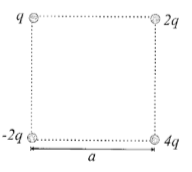
\includegraphics[width=4cm]{Electroestática/Potencial_electrico/p4_potencial.png}
\centering
\end{figure}

\begin{enumerate}[label=\alph*)]
    \item Calcule el trabajo necesario para disponer las cuatro cargas en la configuración mostrada.
    \item ¿Que representa el trabajo?
\end{enumerate}


\newpage